\documentclass[conference]{IEEEtran}
\usepackage[utf8]{inputenc}
\usepackage{amsfonts}
\usepackage{caption}
\usepackage{graphicx}
\usepackage{textcomp}
\usepackage{listings}
\lstset{
    basicstyle=\scriptsize\ttfamily,
    keywordstyle=\color{blue}\ttfamily,
    stringstyle=\color{red}\ttfamily,
    commentstyle=\color{green}\ttfamily,
    breaklines=true
}
\usepackage{url}

% correct bad hyphenation here
\hyphenation{op-tical net-works semi-conduc-tor}

\begin{document}
\title{Relatório - EP4}

\author{\IEEEauthorblockN{Tiago Koji Castro Shibata - 8988730}
\IEEEauthorblockA{Escola Politécnica\\
Universidade de São Paulo\\
tiago.shibata@usp.br}
}

\maketitle

\section{Introdução}
Esse relatório acompanha o quarto exercício programa (EP4) da disciplina PCS3556 - Lógica Computacional. Nesse exercício programa, é implementado o algoritmo de conversão de gramática livre de contexto em forma normal de Chomsky. Em seguida, é implementado um algoritmo de reconhecimento de sentenças utilizando programação dinâmica, a partir da forma normal de Chomsky.

\hfill 21 de Abril de 2018

\section{Tarefa}

Como estudado na disciplina, algumas gramáticas são livres de contexto. A manipulação delas é mais simples: escrever reconhecedores de dadas gramáticas é muito mais fácil e existem algoritmos rápidos de reconhecimento.

Para facilitar o reconhecimento, pode ser usada uma forma normal, como a forma normal de Chomsky. Uma característica importante da forma normal de Chomsky é que toda gramática em forma normal de Chomsky é livre de contexto, e toda gramática livre de contexto pode ser convertida a uma gramática equivalente em forma normal de Chomsky (no entanto, no processo de conversão regras são adicionadas, e a gramática normalizada pode possuir tamanho até o quadrado do número de regras da gramática original, no pior caso. A facilidade de reconhecimento na forma normal pode implicar em maior dificuldade de leitura e compreensão da gramática por um humano).

Uma gramática livre de contexto $G$ é dita em forma normal de Chomsky se todas as suas regras de produção são da forma:

\

$A \to BC$, ou

$A \to a$, ou

$S \to \varepsilon$

\

Onde $A$, $B$, e $C$ são símbolos não terminais, $a$ é um símbolo terminal, $S$ é o símbolo não terminal inicial, e $\varepsilon$ é a cadeia vazia. $B$ e $C$ também não podem ser o símbolo inicial (representado aqui por $S$) e a regra de produção $S \to \varepsilon$ está disponível apenas se $\varepsilon \in L(G)$, ou seja, a cadeia vazia pertence à linguagem gerada por $G$.

No Exercício Programa 2, trabalhamos com um reconhecedor de linguagens sensíveis ao contexto. Nesse Exercício Programa, apenas linguagens livres de contexto serão cobertas; observando a hierarquia de Chomsky, apenas linguagens regulares e livres de contexto são suportadas:

\begin{minipage}{\linewidth}
    \centering
    \label{chomsky}
    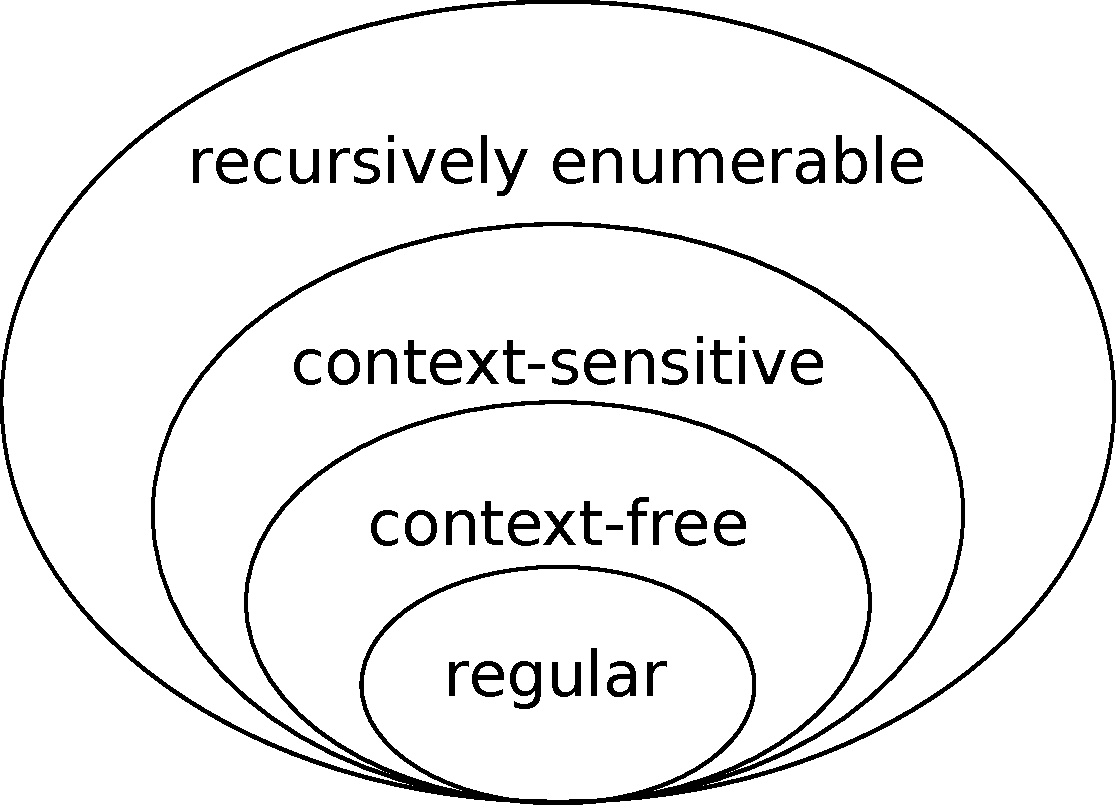
\includegraphics[width=0.8\textwidth]{Chomsky-hierarchy.pdf}
    \captionof{figure}{Hierarquia de Chomsky}
\end{minipage}
\\

Após a conversão para forma normal de Chomsky, implementou-se um algoritmo de reconhecimento com programação dinâmica, muito mais rápido que testar todas as expansões possíveis a partir do não terminal inicial. O algoritmo CYK ou CKY (\emph{Cocke-Kasami-Younger}) \cite{cky} foi escolhido.

\section{Estruturas de dados}

Em alguns locais, estruturas de conjunto fornecidas pelo Elixir (\emph{MapSet}) foram usadas. O uso de conjunto evita que varramos a lista toda para buscar um elemento, e o conjunto permite operações fáceis e rápidas de união ou diferença quando necessário. Funções do módulo \emph{Enum} foram usadas para facilitar a programação funcional.

Nessa implementação, a gramática $G$ é dada como uma tupla \emph{\{regras de produção, símbolo inicial\}}. As regras de produção são dadas como uma lista de tuplas do tipo \emph{\{símbolo inicial, [substituição]\}}. Após conversão para forma normal de Chomsky, todas as regras serão da forma \emph{\{símbolo inicial, [terminal]\}} ou \emph{\{símbolo inicial, [não terminal, não terminal]\}}. Além disso, terminais serão sempre representados por nomes maiúsculos (como \emph{A, NP, ADD}) e não terminais por símbolos ou nomes minúsculos (como \emph{a, he, +}).

\section{Algoritmo - Conversão para forma normal de Chomsky}

Foram implementadas toda a série de operações para transformação em forma normal de Chomsky, baseado no material da disciplina.

Primeiramente, o símbolo inicial foi removido do lado direito de regras de produção, se presente, com adição de um não terminal novo (\emph{S0}), e o código foi testado:

\lstinputlisting{1.ex}

\

\lstinputlisting{1_test.ex}

Depois, terminais presentes no lado direito de regras de produção e não solitários foram substituídos. Cada regra do tipo:

\

$A \to X_1 ... a ... X_n$

\

Foi trocada por um par de regras equivalentes:

\

$N_a \to a$

$A \to X_1 ... N_a ... X_n$

\

Foi implementada a função \emph{eliminate\_nonsolitary\_terminal}, funções auxiliares e testes:

\lstinputlisting{2.ex}

\

\lstinputlisting{2_test.ex}

Depois, regras de produção foram modificadas para possuir no máximo dois não terminais do lado direito. Cada regra do tipo

\

$A \to X_1 X_2 X_3 ... X_n$

\

Foi trocada por regras do tipo:

\

$A \to X_1 A_1,$

$A_1 \to X_2 A_2,$

$... ,$

$A_{n-2} \to X_{n-1} X_n,$

\

Foi implementada a função \emph{eliminate\_right\_side\_with\_multiple\_nonterminals}, funções auxiliares e testes:

\lstinputlisting{3.ex}

\

\lstinputlisting{3_test.ex}

Regras vazias foram reescritas, propagando o não terminal possivelmente vazio para todas as regras que o possuem no lado direito, e apagando a regra vazia:

Foi implementada a função \emph{eliminate\_empty\_rules}, funções auxiliares e testes:

\lstinputlisting{4.ex}

\

\lstinputlisting{4_test.ex}

Foi implementada a remoção de regras de produção unitárias (do tipo $A \to B$, onde $A$ e $B$ são não terminais). Regras do tipo:

\

$A \to B$

\

Com $A$ e $B$ não terminais, foram removidas, e para todas as regras do tipo

\

$B \to X_1 ... X_n$

\

Foi adicionada uma regra do tipo:

\

$A \to X_1 ... X_n$

\

Representando a regra removida de A para B. Iniciou-se com uma implementação simples, que buscava regras unitárias e realizava as substituições:

\lstinputlisting{5_test.ex}

Mas percebeu-se que a implementação falhava em regras unitárias encadeadas (como $A \to B \to C$), dependendo da sequência de aplicação. Foi refeita a implementação, dessa vez buscando se a as novas regras adicionadas possuiam ainda novas regras de produção unitárias, e testes foram escritos:

\lstinputlisting{5.ex}

\

\lstinputlisting{5_test.ex}

Por fim, foi implementada a função \emph{to\_chomsky\_nf}, que chama cada uma das funções anteriores, e mais testes foram escritos:

\lstinputlisting{6.ex}

\

\lstinputlisting{6_test.ex}

\section{Algoritmo - CKY}

Depois, implementou-se CKY. O algoritmo opera de forma \emph{bottom-up}, iniciando por cada caractere da sentença sendo analizada e subindo até gerar a sentença completa. Resumidamente, o algoritmo:

\begin{enumerate}
    \item Varre a cadeia de entrada, e para cada caractere $c$ busca alguma regra $R \to c$ correspondente. Todos os não terminais que podem produzir $c$ são salvos em uma lista.
    \item Agrupa pares de caracteres da sentença: Para cada par de não terminais adjacentes gerados no passo anterior, busca se alguma regra pode produzir o par, e salva em outra lista.
    \item Agrupa trios de caracteres da sequência: Busca regras que gerem um não terminal gerado no passo 1 seguido de um não terminal gerado no passo 2 (ou seja, um não terminal que engloba 3 caracteres da sentença sendo analizada) ou um não terminal gerado no passo 2 seguido de um não terminal gerado no passo 1.
    \item Agrupa quartetos de caracteres da sequência: Busca regras que gerem um não terminal gerado no passo 1 seguido de um não terminal gerado no passo 3 ou dois não terminais gerados no passo 2.
\end{enumerate}

Observa-se que para agrupar $n$ caracteres a partir de estados já processados, são feitos $n - 1$ testes em janelas da sequência (ou seja, para agrupar 4 caracteres da sequência de entrada, são testados os agrupamentos de 1 e 3 caracteres, 2 e 2, e 3 e 1).

Mais detalhes sobre o funcionamento do algoritmo podem ser vistos na referência indicada \cite{cky}. O comportamento \emph{bottom-up} do algoritmo pode ser visto na seguinte imagem, onde o processamento inicia caractere por caractere, agrupando-os até chegar ao símbolo inicial:

\begin{minipage}{\linewidth}
    \centering
    \label{chomsky}
    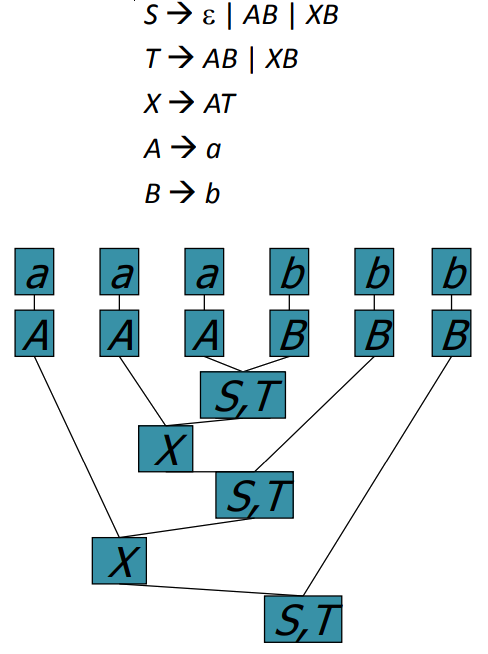
\includegraphics[width=0.8\textwidth]{cky_tree.png}
    \captionof{figure}{Comportamento \emph{bottom-up} do CKY}
\end{minipage}

\

O algoritmo comumente utiliza uma tabela de aplicação de símbolos, subindo na tabela conforme aumenta-se o número de caracteres englobados da cadeia sendo analisada:

\begin{minipage}{\linewidth}
    \centering
    \label{chomsky}
    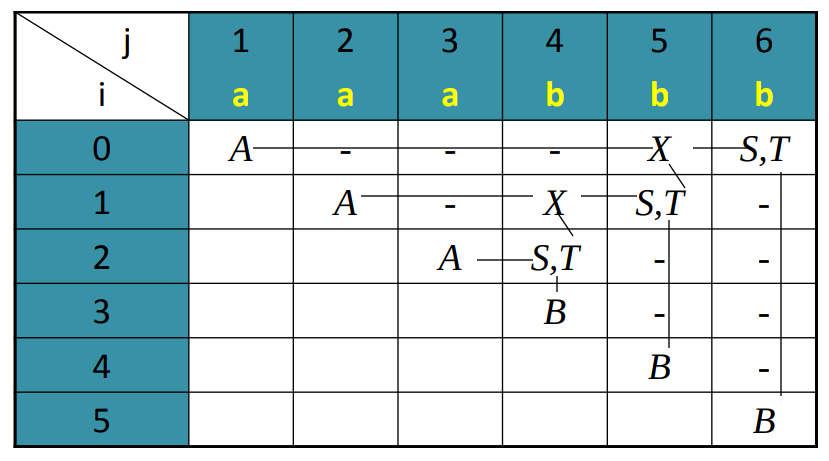
\includegraphics[width=0.8\textwidth]{cky_table.png}
    \captionof{figure}{Tabela do CKY}
\end{minipage}

\

Na minha implementação, utilizei uma matriz implementada como uma lista de listas. A posição $[a][b]$ da matriz indica a subcadeia de comprimento $a$ iniciando em $b$. Cada item da matriz é um conjunto (\emph{MapSet}) de não terminais que podem gerar a subcadeia.

Foi criada uma função para inicializar a tabela CKY. Para isso, a função busca regras que gerem cada terminal da cadeia e os coloca no primeiro item da lista, seguido da tabela vazia. Foram feitos testes:

\lstinputlisting{7.ex}

\

\lstinputlisting{7_test.ex}

Foi feita a função de atualização da tabela:

\lstinputlisting{8.ex}

E a função \emph{cky} principal, com testes:

\lstinputlisting{9.ex}

\

\lstinputlisting{9_test.ex}

\section{Resultados}

A implementação foi um sucesso e passou nos testes realizados. Foram realizados testes com gramáticas longas e complexas, como análise da estrutura de frases simples, e o código funcionou como esperado.

\section{Conclusão}

Pude aplicar os conhecimentos da disciplina em um problema prático e realizar a transformação de qualquer gramática livre de contexto em uma gramática equivalente, em forma normal de Chomsky. Além disso, implementei um algoritmo rápido de reconhecimento de cadeias usando gramáticas normalizadas em forma normal de Chomsky, utilizando programação dinâmica.

\begin{thebibliography}{1}
\bibitem{elixir}
Friedel Ziegelmayer. \emph{Elixir ExDoc}. \url{https://hexdocs.pm/elixir/}, acessado em 12/04/2018
\bibitem{cky}
Scott Farrar. \emph{CKY Algorithm}. CLMA, University of Washington. \url{http://courses.washington.edu/ling571/ling571_fall_2010/slides/cky_cnf.pdf}, acessado em 12/04/2018
\end{thebibliography}

\end{document}
